\chapter{Windows}
\label{chap:windows}

Due to the continuous and infinite characteristics of streaming data, 
it might be impossible to process all data in memory. Therefore, 
stream processing engines utilize buffers to hold the most recent stream of 
records in memory. These buffers are called \emph{windows}. Windows make it 
possible to apply streaming versions of traditional data processing operators such
as joins~\cite{grubjoin}, sorts and aggregations. 

The behaviour of \emph{windows} are configured by specifying \emph{policies}
based on different characteristics such as \emph{count}, \emph{attribute-delta}, \emph{time}, and
\emph{punctuation}~\cite{generic_window_sem}. For this thesis, only a
\emph{time}-based policy is of interest to proof and evaluate the 
concept, specifically with the notion of \emph{event time},
since we are dealing with streaming data with 
timeliness.
\gh{Here we need a good motivation why we limit the scope to the time characteristic.
       I can imagine a use case where we generate triples only if there are 5 particular
records encountered (so count based, e.g. a thermometer signals a high temperature which might trigger an alert). A reason can be to proof the concept, and then later in the discussions / future work section say that 
the concept could also be investigated for other characteristics as well.}

Moreover, the configurations of the policies will be based on the 
implementations in Apache Flink and will differ from those defined by 
Bugra Gedik~\cite{generic_window_sem}. 


To understand the different \emph{windows} and \emph{policies}, we will elaborate on them 
in the following sections. First, a few basic notations will be defined to 
help in the description of the semantic behaviour of the different 
\emph{windows} and \emph{policies}. Secondly, we will describe the mechanism of the 
different windows \textbf{with the semantic implication} imposed by the 
\emph{time}-based \emph{eviction} and \emph{trigger} policies. 
Finally, a review of different state-of-the art custom window operations 
will be discussed to aid us in the development of our methodology for 
dynamic window processing. 


\section{Window Preliminaries}%
\label{sec:window_notations}

Before discussing different \emph{window} types, we will introduce a 
few definitions and notations to describe \emph{windows} based 
on the notations used in~\cite{generic_window_sem}. These notations and definitions 
will be used to aid in explaining different semantic behaviour of the \emph{windows} under 
different \emph{policies}. 

\paragraph{Notations}%
$W = \{r_i | i \in [0\dots|W| - 1] \} $ is a window, whose size is denoted by $|W|$ in terms 
of the number of records inside the window $W$, and $r_i$ as the $i$th record inside 
the window. The records $r_i$ are orderd from the newest to the oldest starting from 
$0\dots n$ with the oldest record being $r_n$ with $ n = |W| - 1$. The current record to be put 
into the window is denoted as $r_c$. The event timestamp associated with the
record $r_i$ is denoted as $\tau(r_i)$.

\section{Window Types}

According to Bugra Gedik~\cite{generic_window_sem}, windows could be categorized into 
three different types; \emph{tumbling} windows, 
\emph{sliding} windows~\cite{stream_standford,spade_stream}, and \emph{partitioned} windows.

\emph{Tumbling} and \emph{sliding} windows are also commonly provided as 
 default window types by stream processing engines. 
They offer the most flexibility in customization with \emph{windows parameters} to fit 
most of the use cases.
\emph{Partitioned} windows are special variations of the \emph{tumbling} and
\emph{sliding} windows, where a partitioned window consists of different sub-windows of same size. 
This enables \emph{multiplexed processing} where independent computations are done across the 
different sub-windows at the same time, resulting in a higher throughput due to 
the parallelization of the processing~\cite{generic_window_sem}.

\subsection{Tumbling Window}%
\label{sec:Tumbling Window}
Tumbling windows have a \emph{fixed} window size and do not 
overlap. The size of the window influences 
the number of elements residing in the window. It stores the elements 
until the window is \emph{full} and this is determined by the \emph{eviction} policy. 
In the context of this thesis, the \emph{size} of the window will be defined by 
a time period bounded by a lower and a higher event timestamp. 

Processing of the elements within the window happens only when a \emph{trigger}
event is fired. This is determined by the \emph{trigger} policy which fires the 
\emph{trigger} event. For tumbling windows, the default \emph{trigger} policy is 
fulfilled when the window is \emph{full}.


\paragraph{Eviction}%
Extending the notations used in Section~\ref{sec:window_notations}, we define 
the event time based tumbling window $W = \{r_t |  t \in \tau(r_0) \dots \tau(r_n) \}$. 
Then, the size of the window is $|W| = [\tau(r_l), \tau(r_h)[$, where  
$\tau(r_l)$ and $\tau(r_h)$ represents the lower and the upper bound of the 
records timestamp respectively. 
The current record $r_c$ must have a timestamp  $\tau(r_l) \le \tau(r_c) \le \tau(r_h)$ 
to be accepted by the window. If $\tau(r_c) \ge \tau(r_h)$, the record will be 
considered \emph{late} as described in watermarking mechanism in Section~\ref{sub:Out of order processing}. 


Since tumbling windows are processed only when the window is \emph{full}, \emph{trigger} events 
are fired at the same time as \emph{eviction} events for tumbling windows.


\subsection{Sliding Window}%
\label{sec:Sliding Window}
Similar to tumbling windows, sliding windows also have a \emph{fixed} window size 
that is immutable throughout the lifetime of a stream processing job. 
In addition to the window size as a parameter, one could also specify the 
\emph{window slide} for sliding window. This parameter specifies how frequently 
a sliding window is created. 
Therefore, if the \emph{window slide} is smaller 
than the \emph{size} of the window, an overlap will be formed and multiple 
windows could exists at that point of time. The records in the overlapped region 
will have to be copied across multiple overlapping windows. 
Taking the \emph{slide} and the \emph{size} into account, we could conclude that 
a tumbling window is a special case of a sliding window where the \emph{slide} is 
equal to the \emph{size} of the window.

Due to the overlapping of windows, extra checks have to be considered 
when evicting the elements in sliding windows, to ensure that the elements in 
overlapping windows are not removed from multiple windows. To overcome this overhead 
of checking when evicting the window, 
stream processing engines copy records across overlapping windows. 
This reduces processing time and latency at the cost of higher memory consumption.

The \textbf{two \emph{policies}} for the sliding windows are the same as those for the \emph{tumbling} windows. 

\begin{figure}[htpb]
    \centering
    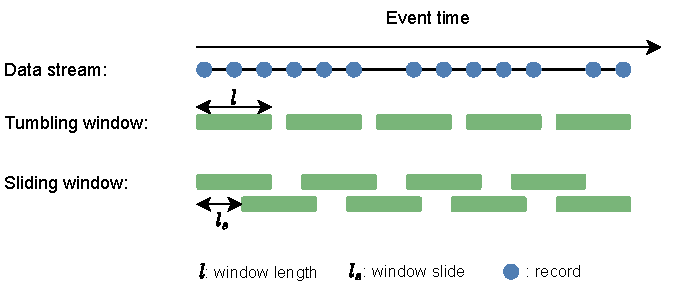
\includegraphics[width=0.8\linewidth]{fig/slide_tumb_windows.pdf}
    \caption{Sliding and tumbling window applied on a data stream~\cite{jonas_scotty}. }%
    \label{fig:slide_tumb_window}
\end{figure}


\subsection{Partitioned Window}%
\label{sec:Partitioned Window}

Unlike the aforementioned window types, where windowing is applied on the stream 
without any changes to the stream, partitioned windows split the data stream into 
different substreams based on the \emph{key} of the partition. This enables 
techniques of \emph{multiplexed processing} to be applied on the data stream, increasing 
the parallelization of stream processing engines. 

\paragraph{Multiplexed processing}%
\label{par:Multiplexed processing}
Most data streams can be split up into multiple substreams consisting of records 
with the same \emph{key} attributes. This is akin to 
the \emph{groupBy} operations present in the traditional batch data processing where 
data records are grouped according to the values of a specific set of the records' \emph{attributes}.
For example, consider a stream containing 
Twitter tweets~\footnote{Twitter API: \href{https://developer.twitter.com/en/docs/twitter-api/v1/data-dictionary/object-model/tweet}
{Twitter's tweet object model documentation.}}. This stream of \emph{tweets} can be 
partitioned into substreams based on the user's id. 
Therefore, to support multiplex processing, any operator applied on the substreams 
must be local to that particular substream. The operators also need to keep the states for each 
substream independently. 


Partitioned windows support \emph{multiplexed processing}, since it consists of  
multiple subwindows; each corresponding to a particular substream identified 
by the \emph{key} attributes of the records in the data stream. The subwindows 
are independent from each other and all computations on the records are in the local scope 
of the subwindow. The actual subwindow semantics can be of the aforementioned window types, \emph{tumbling windows} or \emph{sliding windows}. Therefore, the 
\emph{eviction} and \emph{trigger} policies of the subwindows 
are similar to those two types of windows. 


\begin{figure}[htpb]
    \centering
    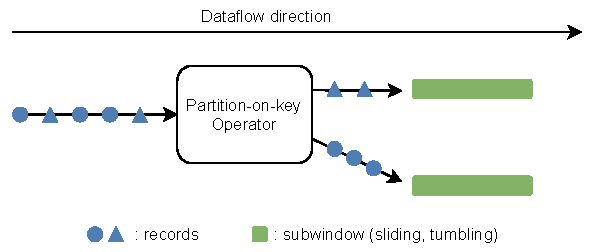
\includegraphics[width=0.8\linewidth]{fig/partitioned_window.pdf}
    \caption{Partitioned window where the records are keyed by an attribute. In this case,
    records are keyed by their shape. After \emph{keying} the records, circle records are sent 
    to another subwindow than triangle records.}%
    \label{fig:partitioned_window}
\end{figure}
   

\section{Windows processing}
\label{sec:windows_processing}

Streaming applications require some form of queries to be executed over 
the data stream. Joins and aggregations are some of the most common queries 
in stream processing which we will elaborate on in the upcoming sections. 

\subsection{Aggregation}%
\label{sub:Aggregation}
Window aggregation is a class of operations where some form of computation 
is done on a group of records within a window. Operations like 
finding the \emph{maximum value} or \emph{average value} are some 
aggregations frequently done in data stream processing. However, 
aggregate operations can be expensive in some situations. 
For example, aggregation operations are expensive when there is 
an overlap of windows (sliding windows), since aggregations over the overlapping 
records will need to be recomputed for each overlapping windows. Given a sliding 
window of 1 minute \emph{size} and 1 seconds \emph{slide}, 60 windows will exist 
at any point of time and the 59 seconds worth of records aggregation will need 
to be recomputed whenever a window receives a \emph{trigger} event for processing. 
This results in redundant computation. 

Optimizing aggregation queries 
on windows has been extensively studied. Jonas et al~\cite{scotty, jonas_scotty} have come up with a method to 
apply generic window \emph{slicing} for optimizing aggregation operators in windows. 
The data stream is modelled as \emph{slices}, where 
records are assigned to exactly one \emph{slice} resulting in a 
$O(1)$ complexity for memory. The \emph{slices} are created every time a 
window begins or ends. Partial aggregations are then applied on the 
records within the slices which will eventually be consolidated once 
a window ends for a final aggregation result eliminating redundant 
computations. According to the authors~\cite{jonas_scotty}, this maintains 
the high throughput processing capabilities of Apache Flink even if the 
number of overlapping concurrent windows increases. 


\subsection{Join}%
\label{sub:Join}

Join operations are different from aggregations. We do not need 
to wait for the window to be full, before processing the records inside the 
window. A \emph{trigger} event could be fired at the very moment a new 
record arrives in the window. Furthermore, multiple statistical approaches 
could be applied for windows optimization without disturbing the results 
of the join operations significantly. Several studies have been conducted to 
improve the join algorithms in windows~\cite{vctw_join, join_tracking, grubjoin, approximate_window_sem, approx_window}. 
The approaches in ~\cite{grubjoin, approximate_window_sem, approx_window} are based 
on dropping some of the records to be joined through \emph{load shedding}. 
Load shedding is a technique to drop the record if 
it fails to meet the conditions specified 
by a metric specific to the implementations. Approaches in ~\cite{grubjoin, approximate_window_sem, approx_window}
assume that the stream is not out-of-order with centralized execution for 
windows processing. Additionally, histograms of the attributes of the records are used, 
either per window or per stream, 
to calculate the threshold for dropping records, inflicting an overhead to memory. 
This leads to higher latency and computation overhead 
when joining records from multiple streams. Furthermore, 
these approaches only deal with \emph{join} operators and could not be applied to other 
types of stream processing operators such as \emph{aggregations} and \emph{reductions}.

VC-TWJoin~\cite{vctw_join} approaches the problem differently by only considering 
the behaviour of the data stream. The approach adjusts the size of the window 
after every \emph{eviction} trigger based on the stream rate. This simple approach 
of dynamically adjusting window sizes, enables load-shedding without the overhead of 
keeping statistical data. Since the metric used by the approach does not use 
record attributes, it has no impact on the calculation 
done by other operators such as \emph{aggregation} and \emph{reduction}.
However, the approach is unstable when the data stream has periodic bursts of data.
It either increases or decreases the size of the window when the metric triggers 
the threshold of the algorithm. At worst case, it can lead to cyclic increase and 
decrease of window sizes, if the metric borders around the threshold with every 
update of the metric.


\section{Summary}%
\label{sec:Summary}

The aforementioned window types are fixed and are not robust to changes of the data stream characteristics. Once initialized, the windows sizes 
are fixed throughout the runtime of the application. This results in inefficient 
window sizes if the data stream rate diverges greatly over time; a window size might become too small to process the incoming 
data. Thus, a dynamic window that adjust its size throughout the runtime of the application 
will adapt better to the changing characteristics of the data stream. 


